%
% This contains critical information regarding the burn, things like location,
% where the nearest hospital is located, definitions of terms, acronyms, the rules, 
% and information on any other burn-related resources.
%%
% This contains critical information regarding the burn, things like location,
% where the nearest hospital is located, definitions of terms, acronyms, the rules, 
% and information on any other burn-related resources.
%

\chapter{Astronaut Training}

\section*{Guidelines}
We have few rules and kindly ask you to follow them, for your safety and those around and with you.  Look at them as a compass to orient yourself by while drifting in the orbit of this event. 

\subsection*{Safety}
Safety is our number one concern and breaching perimeter is a \textbf{serious} offense we will handle swiftly. 

\subsubsection*{Fire Safety}
\begin{itemize}[noitemsep]
\item \textbf{\textcolor{red}{If you breach effigy or temple perimeter, you will be removed from the property immediately -- no questions asked!}} 
\item No open ground and / or unattended fires. They must be contained and off ground. Please bring a fire bowl for this purpose. If you see a fire that is unattended or out of control, contact a Ranger immediately.
\end{itemize}

\subsubsection*{River Safety}
\begin{itemize}[noitemsep]
  \item Children under 13 must wear a flotation device.
  \item Children under 13 must wear water shoes (water shoes are highly recommended for  \textbf{Anyone} for added safety and traction, especially if caught in a current).
  \item All minors must be accompanied by a parent or legal guardian when in the water.
  \item \textbf{Anyone caught committing the below two actions will be ejected from the burn immediately:}
  \begin{itemize}[noitemsep]
    \item No jumping or diving off the bank into the river.
    \item No swimming after dark.
  \end{itemize}
\end{itemize}

\begin{figure}[H]
\centering
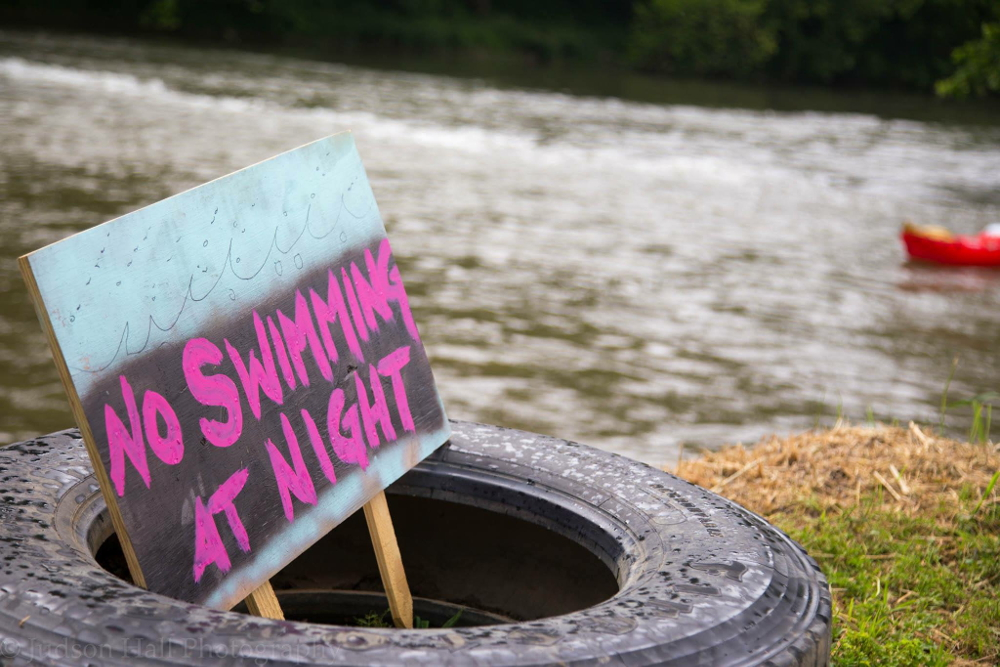
\includegraphics[width=.3\textwidth]{images/riversafety.jpeg}
\caption{No swimming at night. Image courtesy of Judson Hall Photography, 2016.}
\label{fig:2016riversafety}
\end{figure}

\clearpage
\subsection*{No Pets}
\label{sub:nopets}

Spirit Crossing has a \textbf{no pet} policy!

Should you need a service animal’s assistance to safely navigate our premises, please let us know at the gate.  A ``service animal'' is a dog (or other animal) individually trained to do work or perform certain tasks for a person with a disability.

Please be prepared to answer the following two questions so we may better determine at our discretion if your animal falls under the Service Animal Category, and in order for us to be in compliance with ADA regulations:

\begin{itemize}[noitemsep]
\item Is the service animal to the direct benefit of the disability?
\item What tasks and what work is the animal trained to perform in direct relation to the disability? 
\end{itemize}
 
If your animal falls under one of the following categories, you will not be able to bring it into the festival grounds.

Service Animals are \textbf{not}:
\begin{multicols}{2}
\begin{itemize}[noitemsep]
  \item emotional support animals
  \item therapeutic animals
  \item companion animals
  \item comfort animals
  \item service animals in training
\end{itemize}
\end{multicols}

For your convenience, Scooby Shack Kennel is 20 minutes from Sneedville and can be reached at 423-921-0611.

Thank you for your cooperation and understanding!

\begin{figure}[H]
\centering
	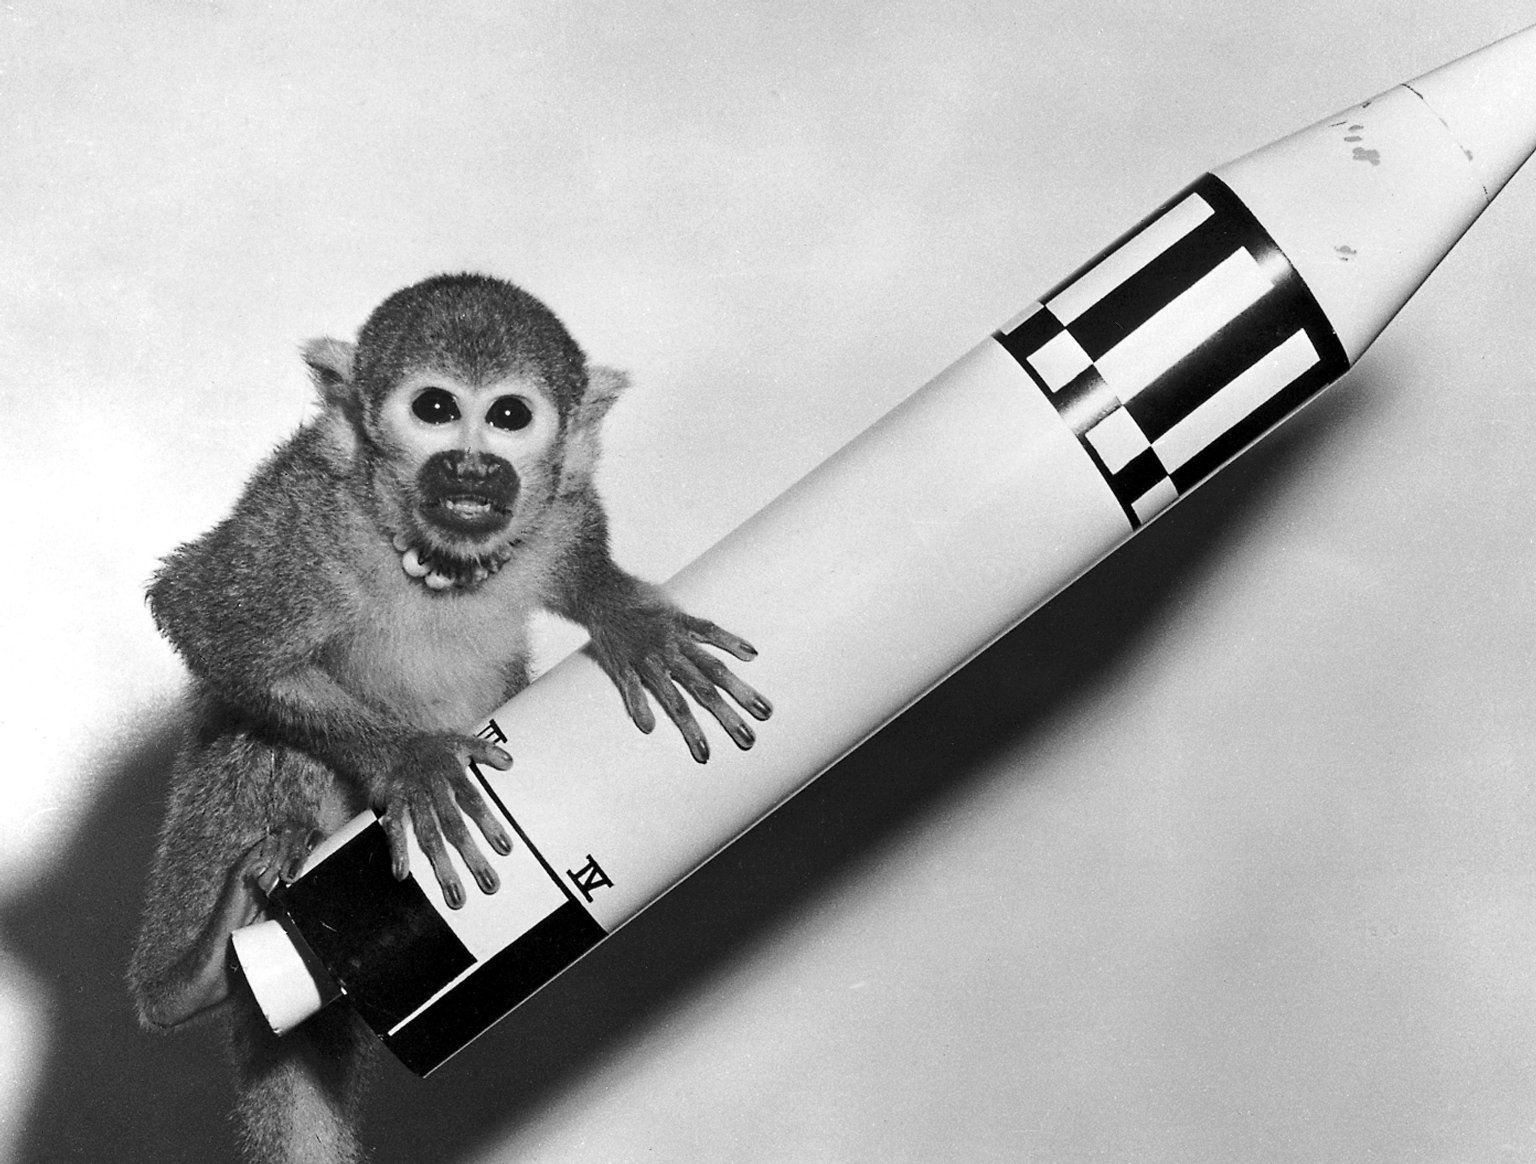
\includegraphics[width=.7\textwidth]{images/Baker}
    \caption{Miss Baker was a squirrel monkey who went into space and back in 1959. This is her on a model of Jupiter AM-18, the rocket that took her into space.}
    \label{image:missbaker}
\end{figure}

\clearpage
\subsection*{Respect the Laws of the Land}
Spirit Crossing, and Sneedville, are kind enough to be our home.  Here are some helpful tips on respect:
\begin{itemize}[noitemsep]
\item While the porch and patio may be used for specific team lead functions, the property owner’s house is off limits to participants.  Please be respectful of the land and grounds.
\item Although held on private property, TN Nudity Laws still apply.  To The Moon is an all ages event so please plan on wearing pasties, bikinis, loincloths, etc.
\item Please respect the land, the river, and the community.  Obey the speed limits and be courteous to those around you.
\item When in doubt, practice \textbf{consent}!
\item TTM  is an all ages event.  Those who are 21 or older will have a special wrist band indicating that they are able to legally consume alcohol. Please consume in moderation.
\end{itemize}
    
\begin{multicols}{2}

% \subsection*{Alcohol}
% \gls{ttm} is an all ages event.  Those who are 21 or older will have a special wrist band indicating that they are able to legally consume alcohol.

\subsection*{Camping}
You may not camp in your car. Please bring a tent or RV / trailer.
Cars may only be brought on site with approval.
% \bod[inline]{needs vetting}

\subsection*{Code of Conduct}
\Gls{ttm} now has a Code of Conduct. You can find it on page~\pageref{coc}.

\subsection*{Fireworks and Effects}
Fire effects with registered Theme Camps only, please.

\subsection*{\Gls{gifting}}\label{gifting}
This is a gifting community, providing refuge from everyday societal perils.  Once you're inside, no commercial activity takes place. Which is part of the charm, and the point :) 
Sometimes, there is a bit of a misconception of "Oh, so it's a barter system?" -- Actually, it's not. It's a "Gifting" Principle.
You gift without the expectation of a gift in return. 
You gift something to someone because at that moment, you feel the other person should have the very thing you'd like to give.

\subsection*{\Gls{graywater}}
There are no plans to dispose of gray water on site.  Each participant is responsible for \gls{pipo}.

% \subsection*{Nudity}
% TN Nudity Laws prohibit full or partial nudity on public property, and while we are on private property, the road cutting through Spirit Crossing is public, mostly accessed by residents, so very low traffic.

% We recommend you use discretion and wear pasties, paint, bikinis, etc.

\subsection*{Minors}
Minors must be accompanied by a parent or legal guardian. If they cause problems during the event which lead to possible safety issues or are a severe nuisance to others, we may ask you to remove the offending minor, possibly your entire camp. Minors are NOT allowed to use, play with, operate nor hold fire, fire props, fire effects and pyro, including poofers.  

%\subsection*{Public Health and Safety}

\subsection*{Recharging batteries for medical equipment}
Those with CPAPs and electronic scooters will have to make their own arrangements to recharge batteries.  \gls{ttm} does not provide battery recharging stations for medical equipment.

Some theme camps have generators, and may allow use of a spare generator plug for recharging medical equipment as a way of \gls{gifting}.  Home Depot and other companies also rent generators.  Moreover, there exist solar panels for recharging CPAP machines, though those can be prohibitively expensive.

% Not that this is now elsewhere in the document in the section on landing/exiting/etc.
% There is now also an explicit table that breaks down the gate hours by day.
% \subsection*{Re-Entry}
% Gate hours will be strictly adhered to unless prior arrangements have been made with event lead and / or property owner.
% Re-entry is prohibited unless
% \begin{itemize}[noitemsep]
% \item for medical reasons
% \item prior arrangements have been made
% % \item another invite is purchased 
% \end{itemize}
% Gate hours are 10 a.m. -- 10 p.m. Thursday and Friday, and 10 a.m. -- 6 p.m. Saturday.
% \bod[inline]{Are these hours correct? I got them off of a Dusty comment on Facebook.}

% \subsection*{Respect}
% Please respect the land, obey the speed limits, and be courteous to those around you.



\columnbreak
\subsection*{Photography}
Please respect the right of others who may not wish to be photographed. Ask \textbf{permission}! If you see someone with a \textcolor{blue}{blue} wristband, that is a \textbf{no photo} policy indicator. 
Do not take pictures or video of participants wearing them! 

% \subsection*{Property Owner's House}
% \todo[inline]{Home Base is not mentioned in the glossary. Is this the correct name?  And aren't the greeters near the site entrance?}
% While the porch and patio are used for \gls{greeter} Station and Home Base, the house is off limits to participants.  Please be respectful of the land and grounds. 

\subsection*{Sound}
To make this event enjoyable for all, amplified sound is limited to 300 Watts producing 90 db at 20 feet. All amplified sound is to be reduced after 4\am nightly to allow room for acoustic and ambient sound and to limit the possibility of neighboring sound complaints. 

\subsection*{Wristbands}
\label{sub:wristbands}
% \bod[inline]{needs vetting -- is the gate the correct location?}
You will receive a wristband when you arrive at the \gls{gate}.  Different colored wristbands will identify you as being over 21, under 18, etc.  Wristband colors also indicate if you don't want your photo taken.  

You must keep your wristband on at all times.  See the \gls{gate} if you need to replace your wristband.

\subsection*{Vending}
No vending, selling, or promoting is allowed at the event.
\end{multicols}

% \begin{tabular}{|p{6cm}|p{6cm}|} \hline
% \textbf{Do} & \textbf{Don't} \\ \hline \hline
% Follow safety protocols  & Breach effigy or temple perimeter               \\ \hline
% Camp in a tent or RV &  Camp in your car              \\ \hline
% Limit amplified sound to 90dB at 20 ft  & Bring your car on site+               \\ \hline
% Reduce amplified sound after 4 a.m. & Leave minors unattended               \\ \hline
% Obey TN nudity laws (cover up) & Sell, vend, or promote               \\ \hline
% Stay out of the property owner's house  & Leave fires unattended               \\ \hline
% Use fire bowls  & Start open ground fires               \\ \hline
% Respect land and neighbors  & Put anything but 1-ply toilet paper and human waste in portapotties               \\ \hline
% Ask permission before taking photos  & Take pictures of participants with green wristbands               \\ \hline
% Ask for consent  &   \\ \hline             
% \end{tabular}
% \vspace{2em}



\section*{Community Standards}

\subsection*{The Ten Principles}\label{tenprinciples}
Table \ref{tbl:tenprincples} enumerates the 10 Principles of \gls{ttm}.
Funny thing about those: they are not meant to be chosen at random to suit ones need, mood or agenda, but according to our interpretation were created to work together as a whole.  
Meaning your right to radically and freely express yourself ends when your expression infringes upon another participant to do the same. 

In other words, they're not a "Getting out of jail free" card, nor a permission slip to be a dick. So don't be a dick, hiding behind one or two principles. 

\begin{center}
	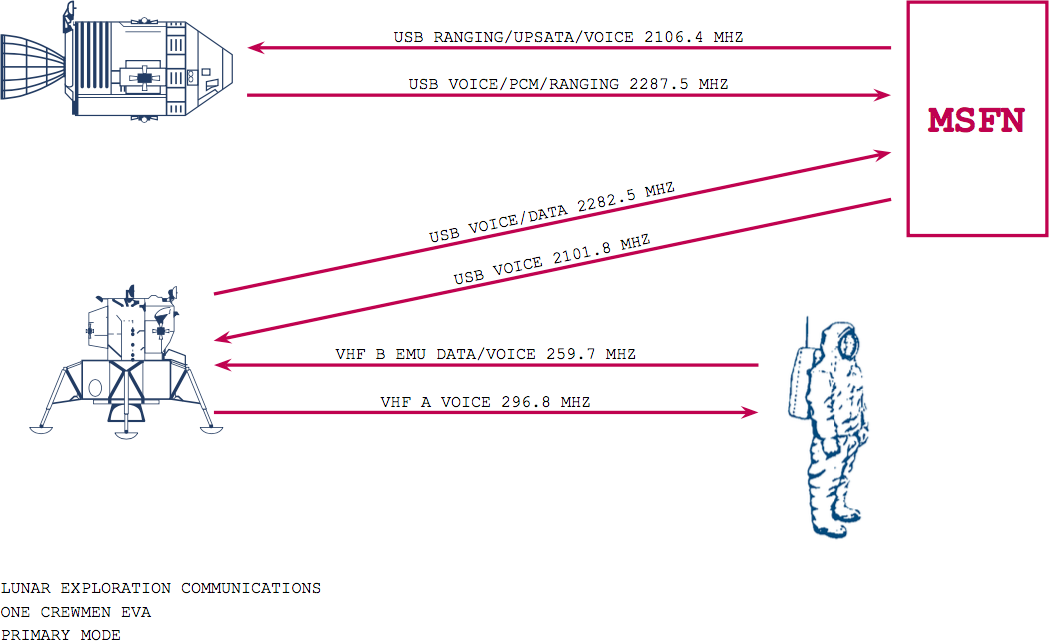
\includegraphics[width=.7\textwidth]{images/communication2}
\end{center}

\vspace*{\fill}
\begin{table}[h!]
\footnotesize
\centering
\caption[The 10 Principles]{The 10 Principles}
\label{tbl:tenprincples}
\begin{tabular}{@{}llp{4.3in}@{}}
\toprule
\textbf{No.} & \textbf{Principle}               & \textbf{Description}                                 \\ \midrule
1   & Radical Inclusion       & Everyone is welcome, all types, all kinds, friends, strangers, and in between.         \\[1em]
2   & Gifting                 & Gifts are unconditional offerings, whether material, service oriented, or even less tangible. Gifting does not ask for a return or an exchange for something else.        \\[1em]
3   & Decommodification       & Hand in hand with gifting, burns are environments with no commercial transactions or advertising. Nothing is for sale - we participate rather than consume.        \\[1em]
4   & Radical Self-Reliance   & You are responsible for you. Bring everything with you that you need. Burns are an opportunity for you to enjoy relying on yourself.          \\[1em]
5   & Radical Self-Expression & What are your gifts, talents, and joys? Only you can determine the form of your expression.         \\[1em]
6   & Communal Effort         & Cooperation and collaboration are cornerstones of the burn experience. We cooperate to build social networks, group spaces, and elaborate art, and we work together to support our creations.         \\[1em]
7   & Civic Responsibility    & Civic responsibility involves the agreements that provide for the public welfare and serve to keep society civil. Event organizers take responsibility for communicating these agreements to participants and conducting events in accordance with applicable laws.         \\[1em]
8   & Leaving No Trace        & In an effort to respect the environments where we hold our burns, we commit to leaving no trace of our events after we leave. This means everything that you bring with you goes home with you. Everyone cleans up after themselves, and whenever possible, we leave our hosting places better than we found them.            \\[1em]
9   & Participation           & The radical participation ethic means you are the event. Everyone works; everyone plays. No one is a spectator or consumer.        \\[1em]
10  & Immediacy               & From the Burning Man website : "Immediate experience is, in many ways, the most important touchstone of value in our culture. We seek to overcome barriers that stand between us and a recognition of our inner selves, the reality of those around us, participation in society, and contact with a natural world exceeding human powers. No idea can substitute for this experience."             \\ \bottomrule
\end{tabular}
\end{table}
\vspace*{\fill}


\clearpage
\subsection*{The 11th Principle -- Consent}

\gls{ttm} has adopted the 11th Principle, Consent\footnote{\url{http://www.11thprincipleconsent.org/2015/10/20/what-do-you-consent-to/}}.

\begin{labeling}{Photography:}
	\item[Touch:] Just because you hugged someone yesterday doesn't mean you can surprise them with a hug today. ``Surprise contact'' isn't always wanted, even if it's affectionate.
	\item[Kink:] Consent for one thing isn't consent for another. If I said you can spank me, that doesn't give you permission to grope me.
	\item[Sex:] Consent can be revoked once it's been given.
	\item[Gifts:] Disclose what is in your gifts, even if it's just essential oils. Some people have sensitivities.
	\item[Foods:] Disclose the ingredients, one person's innocuous ingredient can be someone else's allergy.
	\item[Photography:] Ask before taking pictures. Remember consent to take a picture is NOT consent to post it on your blog.
\end{labeling}


\section*{Code of Conduct}\label{coc}
TouchBass LLC / To The Moon Code are introducing a new Code of Conduct for 2018 and beyond.
If you are unable to agree to these terms and our policies, we’ll gladly issue a refund for your ticket.
Please contact us at connect@tothemoonburn.com. 

% \subsection*{The Moon Code Of Conduct}

\begin{multicols}{2}
To The Moon, produced by TouchBass LLC, relies on attendees and volunteers to create and maintain a space that is welcoming for all ticketed participants. We don’t discriminate on gender, sexual orientation, disability, ethnicity, socioeconomic status, age, or religion and we abide by the Burning Man 10 Principles.

Participation in this event is open to all ticketed attendees, but is a privilege nonetheless. Attending privileges of To The Moon and related events sponsored by TouchBass LLC will be revoked if a participant fails to respect other attendees or behaves in a way that endangers themselves, the event, or the broader community as a whole.
Damaging behavior is not limited to violence or consent violations, but rather includes ALL behavior detrimental to The Moon as a whole, the burn itself, affiliated events, TouchBass LLC, its BOD, Team Leads, and volunteers and other participants by means of any actions in direct contradiction to and out of alignment with our mission:

\emph{“To The Moon exists solely to create a platform allowing its participants to unfold their creative wings and embrace and nurture a community striving to share their passions, unique gifts and talents and come together in celebration to do just that.”}

We want to impose upon your freedoms within our chosen community as little as possible, but need to protect our members and event at the same time.
The following are our policies designed to do just that.
If you experienced anything in violation of these guidelines, please fill out our incident report form to help us investigate.

Please note: 3rd Party Incident Reports are not accepted. The report has to be submitted by the person directly involved in / with the incident. If you feel the need to report something as a 3rd Party, please email us at connect@tothemoonburn.com.

\subsection*{Expected behavior includes, but is not limited to}

% \begin{itemize}[noitemsep]
	\subsubsection*{Consent}
    \begin{itemize}[noitemsep]
    	\item Obtaining someone’s consent in a sexual context is absolutely mandatory
        \item Obtaining consent for video or photography of a participant, or in any other way which potentially affects the experience of another person on The Moon is mandatory
	\end{itemize}
        
    \subsubsection*{Non Consensual}
    \begin{itemize}[noitemsep]
        \item Be considerate and respectful of fellow participants and the community around the event.
        \item Refrain from non-consensual demeaning, discriminatory, or harassing behavior.
        \item Be mindful of your surroundings and of your fellow participants’ safety.
	\end{itemize}
% \end{itemize}

\subsection*{Unacceptable behavior includes but is not limited to}
\begin{itemize}[noitemsep]
    \item Predatory behavior, defined as any unwanted and non-consensual form of the following
    \begin{itemize}[noitemsep]
        \item Non-consensual physical contact, including unwelcome sexual interaction
        \item Intimidation, harassment, stalking
        \item Verbal or physical abuse
        \item Spousal abuse
        \item Violence against other participants or their property.
	\end{itemize}
         
    \item Abuse or neglect of To The Moon or land owner’s property, physical or otherwise, such as vandalism, theft of event property
     
    \item Sabotaging To The Moon, its Event Leads and other TouchBass LLC sponsored events, and the BOD by (including but not limited to)
    \begin{itemize}[noitemsep]
        \item Willfully perpetuating false information about TouchBass LLC’s operating procedure
        \item Intentionally damaging relationships fostered by To The Moon for future events by exhibiting aggressive or manipulative behaviors toward hosts and attendees of Touch Bass LLC events
        \item Deliberately harassing BOD members, Team Leads, volunteers or participants for the sole purpose of undermining TouchBass LLC Leadership, its BOD,  operating procedure, events and mission.  
	\end{itemize}

	\item Disrespecting the local community around the event by
    \begin{itemize}[noitemsep]
        \item Dumping trash in local dumpsters
        \item Trespassing
        \item Repeated violations of the event’s sound ordinance
    \end{itemize}

	\item Disregard for one’s own safety (including intentional self harm or intention of) or well-being to such an extent it demands the intervention of other participants, community members, Team and / or Event Leads. volunteers or outside agencies, such as intervention by local law enforcement or fire department staff.
    
	\item Repeated or egregious violations of any and all policies put in effect by event organizers.
    
    \item Defiance against Rangers or other Safety Team Leads, Event Leads and land owner handling a potentially dangerous or life threatening situation.
    
    \item Breaching Perimeter at any effigy / temple burn
\end{itemize}

\subsection*{Consequences of unacceptable behavior}
Unacceptable behavior will not be tolerated. This includes additional forms of said behavior at the burn as well as pre- or post-burn events and via all forms of communication across all platforms.

\textbf{Anyone asked to stop unacceptable behavior is expected to comply immediately.}

Participants who engage in unacceptable behaviors will be subject to event organizers action deemed appropriate to ensure the safety of the event, its affiliate events and affiliate relationships and its participants.
This action may include expulsion from the event without refund, revoking tickets, removing a volunteer from their shift, and temporary or permanent bans from TouchBass LLC events.

If a participant’s behavior does not comply with this code of conduct, does not align with our mission, or puts the future of TouchBass events at risk, (i.e. our burn, Town Halls, Fundraisers) a suspension for the present or following years may be imposed.
Suspensions may not be permanent, and appeals may be submitted in writing in cases where conflict resolution is demonstrated by the offending party. The appeal’s timeline is determined by TouchBass LLc and will be resolved between members of the Board and the suspended party.

TouchBass LLC or individuals may pursue potential legal action.
\end{multicols}

\vspace{2.75cm}

\begin{figure}[!h]
\centering
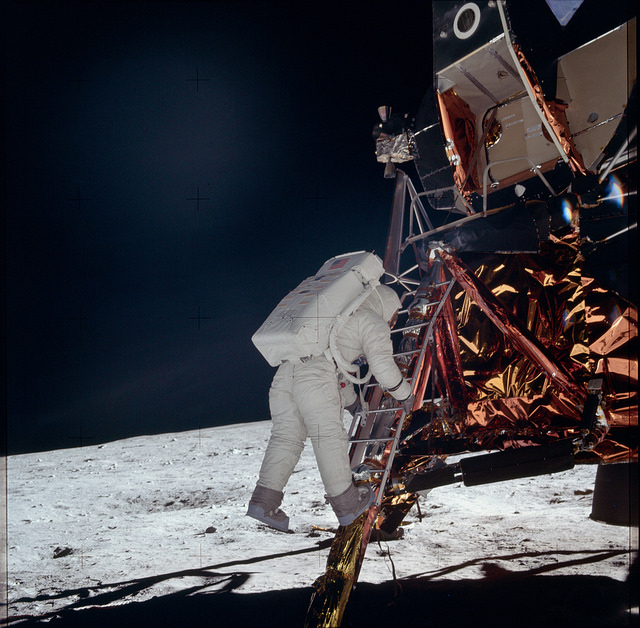
\includegraphics[width=.9\textwidth]{images/arrival.jpg}
% \caption{Astronaut climbing out of the }
\label{image:firststep}
\end{figure}

